\documentclass[a4paper]{article}
\usepackage[utf8]{inputenc}
\usepackage{amsfonts}
\usepackage{amsmath}
\usepackage{amsthm}
\usepackage{graphicx}
\usepackage{array}
\usepackage[footnotesize,bf]{caption}
\usepackage{mathtools}
\usepackage{booktabs}
\usepackage[format=hang]{caption}
\usepackage{subfigure}
\usepackage{textcomp} % For the cent symbol
%\usepackage[font=footnotesize]{subcaption}
\usepackage{varioref}
\captionsetup{justification=justified, singlelinecheck=true}
\usepackage[backend=biber,url=false,doi=false,style=authoryear]{biblatex}
%\addbibresource{D:/Rob/Dropbox/PhD/Writing/bibtex/Zotero - IO Modelling.bib}
%\addbibresource{D:/Rob/Dropbox/PhD/Writing/bibtex/Zotero - Trade.bib}
%\addbibresource{D:/Rob/Dropbox/PhD/Writing/bibtex/Zotero - Networks.bib}
\addbibresource{/home/rob/Dropbox/PhD/Writing/bibtex/Zotero - IO Modelling.bib}
\addbibresource{/home/rob/Dropbox/PhD/Writing/bibtex/Zotero - Trade.bib}
\addbibresource{/home/rob/Dropbox/PhD/Writing/bibtex/Zotero - Networks.bib}
\usepackage{authblk}
\usepackage{attrib}
%\bibliographystyle{elsarticle-harv}
%\nocite{*}
% % Diagramming
\usepackage{tikz}
\usetikzlibrary{arrows,positioning,decorations}
% %

\title{A global inter-country economic model based on linked input-output models \\ DRAFT}
\author[*]{Robert G. Levy}
\author[**]{Thomas P. Ol\'{e}ron Evans}
\author[*]{Alan G. Wilson}

\affil[*]{Centre for Advanced Spatial Analysis, UCL Bartlett Faculty of the Built Environment,
90 Tottenham Court Road, London W1T 4TJ, UK}
\affil[**]{Department of Mathematics, University College London, Gower Street, London WC1E 6BT, UK}


\begin{document}
\maketitle

\begin{abstract}
A global model is presented that can be used as the basis for assessing the impacts of future changes in trade, migration, security and development aid.
The model is based on input-output models for 40 countries, linked with trade data at the sector level.
This is made possible by the World Input-Output Database, a collection of input-output tables for 40 countries across 15 years, and by databases of commodities and services trade from the UN.
The model is constructed using a minimum number of assumptions, and is based as far as possible on empirical observation.
Some initial analysis of the model and its properties are also presented
\end{abstract}

\section{Introduction}
The objective of this paper is to present global economic model that can be used as the basis for assessing the impacts of future changes in trade, migration, security and development aid.
The model presented here represents a first `proof of concept' step towards this ambitious goal.
The economies of individual countries are represented as 35-sector input-output models each of which is linked through trade flows representing imports and exports.
This has recently been made feasible by the publication of the World Input-Output Database (WIOD) \parencite{Timmer2012}, a collection of national input-output tables (NIOTs) for 40 countries across 15 years, from 1995 to 2009.
The NIOTs are linked through data from the UN covering trade in both goods\footnote{comtrade.un.org/db} and services\footnote{unstats.un.org/unsd/servicetrade/}.

The remainder of this paper is structured as follows: 
Section \ref{sec:litreview} gives an overview of existing work in this area.
Section \ref{sec:system} gives a description of the present system and outlines how data is used to calibrate the parameters of the model.
The algorithm used to calculate the output of the model is described in section \ref{sec:algorithm} and some preliminary results are given in section \ref{sec:results}.

Some concluding comments are added in section \ref{sec:conclusions}.

\section{Existing Global Economic Models} \label{sec:litreview}
In the mid-1970s, the creator of input-output economics, Wassily Leontief, had just won the Nobel prize for Economics and took the prestige that this bestowed on him as an opportunity to announce a very ambitious project to model the global economy:

\begin{quotation}
Major efforts are underway to construct a data base for a systematic input-output study not of a single national economy but of the world economy viewed as a system composed of many interrelated parts [...]
Preliminary plans provide for a description of the world economy in terms of twenty-eight groups of countries, with about forty-five productive sectors for each group. \attrib{\cite{Leontief1974}}
\end{quotation}

Some 20 years later, Faye Duchin, a former research assistant of Leontief, described how Leontief's efforts in this area have largely been ignored by economists, describing the departures from the standard, neoclassical modelling in terms of price elasticity and elasticity of substitution as being ``too great to ignore'' \parencite{Duchin2004}. 
See section \ref{sec:iots} for more on this subject.

In the years since Leontief published his global model, input-output analysis has been largely restricted to regional studies, of which \textcite{Akita1993}, \textcite{Khan1999} and \textcite{Luo2013a} are examples; and studies related to energy and the environment, such as  \textcite{Leontief1970}, \textcite{Joshi1999}, \textcite{Bergh2002} and \textcite{Hendrickson2006}.

However, much more recently, attention has returned to input-output modelling in a global context more generally. \textcite{Tukker2013} describe how several multi-regional input-output (MRIO) models have been developed in the very recent literature.
These are, along with the WIOD which is used in the present model, EORA \parencite{Lenzen2012}, EXIOPOL \parencite{Tukker2013a} and the slightly more mature, but proprietorial GTAP \parencite{Walmsley2012}.

Each of these existing models of the global economy extend the idea of the national input-output table to an international setting: where the magnitude of every bilateral sector--sector flow is recorded for a given country in an NIOT, these projects record the magnitude of every country/sector--country/sector flow.
Thus, for example, the extent to which British agriculture purchases from Belgian manufacturing is recorded in dollar amounts.
This results in a very large matrix which, by inverting in the normal input-output way, can be used to predict the impact of a particular exogenous change in demand.
The authors believe that this is taking the simplicity and elegance of input-output analysis a little far; the idea that each sector buys in fixed proportion from each other sector in each other country turns the above-mentioned ignoring of price- and substitution-elasticities from a convenient simplification in the case of the NIOT to an out-and-out denial of the concept of economic dynamics.

The present model provides a framework in which the beauty of input-output analysis at the national level can be combined with a more subtle understanding of the dynamics of international trade.

\section{The System Description} \label{sec:system}
The model presented here has $c$ countries, the economies of which are divided into $s$ productive sectors.
Although each sector produces many distinct goods, these goods are considered to be perfect substitutes, allowing the terms `sector' and `product' to be used interchangeably throughout this paper.
All goods flows are given by value, measured in millions of current price US\$.
For the remainder of this paper the terms `quantity' and `value' will be used interchangeably.
Goods produced domestically are labelled with a dagger superscript ($\dagger$) and imported goods with an asterisk superscript.
Table \ref{tbl:cvars} shows the quantities, taken from data published by the WIOD, which characterise a country's economy for a particular year.
Note that for clarity, no time subscript is added. In future time-series analyses such a subscript would have to be added.

\subsection{Input-Output Tables} \label{sec:iots}
Input-output is, at its heart, an accounting methodology.
The products produced by and imported into a given country in a given year must be either: sold as inputs to other sectors, `intermediate supply'; supplied to the `final demand' of consumers and the government; invested; or exported.
The total amount imported and produced must equal the amount used, consumed, invested and exported for each sector.

By simple summation, total production of sector $s$ in country $i$ can be defined as the sum of all intermediate supply, plus supply to final demand, investment and export:
\begin{equation}\label{eqn:x}
x_s^{(i)}=\sum\limits_{t}z_{s,t}^{\dagger(i)} + f_s^{\dagger(i)} + n_s^{\dagger(i)} + e_s^{(i)}
\end{equation}
where $z_{s,t}^{\dagger(i)}$ is the intermediate supply from domestic sector $s$ to sector $t$ in country $i$, $f_s^{\dagger(i)}$ is final demand for domestic sector $s$, $n_s^{\dagger(i)}$ is investment and $e_s^{(i)}$ are exports.
The total import of sector $s$ in country $i$ is the sum of all intermediate supply by imported goods, plus demand for and investment of imported goods (in this iteration of the model, no imported goods are exported; that is, \textit{re-exports} are set to zero):
\begin{equation}\label{eqn:m}
m_s^{(i)}=\sum\limits_{t}z_{s,t}^{*(i)} + f_s^* + n_s^*
\end{equation}
By assembling these data values in a particular arrangement, an input-output table can be constructed, $\boldsymbol{T}^{(i)}$, as described by \textcite{Miller1985}.
Neglecting the $(i)$ superscript for clarity, the input-output table (IOT) is defined as follows:

\begin{equation}\label{eqn:T}
\begin{array}{rc}
\begin{array}{cc} & \mbox{Sector} \end{array} 
& 
\begin{array}{cccc} \hspace*{4mm}1 & \mathellipsis & s & \hspace*{2mm} \mbox{F.D. Inv Exp Tot} \end{array} \vspace*{2mm} \\
\begin{array}{r}
\begin{array}{rc}
\mbox{Domestic} & \left\{ \begin{array}{c}
1 \\
\vdots \\
s
\end{array} \right. \\
\mbox{Imports} & \left\{ \begin{array}{c}
1 \\
\vdots \\
s \\
\end{array} \right.
\end{array} \vspace*{2mm} \\
%\begin{array}{cc} \hspace*{17mm} & \mbox{Value Added} \end{array}
\end{array} &
\left( \begin{array}{ccccccc}
z^{\dag}_{1,1} & \mathellipsis & z^{\dag}_{1,s} & f^\dag_{1} & n^\dag_{1} & e_{1} & x_1 \\
\vdots & \ddots & \vdots & \vdots & \vdots & \vdots & \vdots \\
z^{\dag}_{s,1} & \mathellipsis & z^{\dag}_{s,s} & f^\dag_{s} & n^\dag_{s} & e_{s} & x_{s} \\
z^*_{1,1} & \mathellipsis & z^*_{1,s} & f^*_{1} & n^*_{1} & 0 & i_1 \\
\vdots & \ddots & \vdots & \vdots & \vdots & \vdots & \vdots \\
z^*_{s,1} & \mathellipsis & z^*_{s,s} & f^*_{s} & n^*_{s} & 0 & i_{s} \vspace*{2mm} \\
%v_{1} & \mathellipsis & v_{s} & 0 & 0 & 0 & G
\end{array} \right)
\end{array}
\end{equation}
Table \ref{tbl:cvars} shows a summary of the quantities used in \eqref{eqn:T}. It will often be convenient to gather those quantities having a single subscript into vectors, and those with two subscripts into matrices. 
\begin{table}
\begin{center}
\begin{tabular}{cl}\toprule
$f_s^{(i)}$ & final demand on sector $s$ in country $i$\\
$n_s^{(i)}$ & investment of sector $s$ in country $i$\\
$e_s^{(i)}$ & export of sector $s$ in country $i$\\
$z_{s,t}^{\dagger(i)}$ & intermediate demand on domestic sector $s$ by sector $t$ in country $i$\\
$z_{s,t}^{*(i)}$ & intermediate demand on import sector $s$ by sector $t$ in country $i$\\\bottomrule
\end{tabular}
\end{center}
\caption{Quantities from data which define a country's economy}\label{tbl:cvars}
\end{table}

We can then characterise a country's economy through the $s$-vectors $\boldsymbol{f}^{(i)}$, $\boldsymbol{n}^{(i)}$ and $\boldsymbol{e}^{(i)}$, and by the $s\times s$ matrices $\boldsymbol{Z}^{\dagger(i)}$ and $\boldsymbol{Z}^{*(i)}$.
In matrix form, $\boldsymbol{T}$ may be written:

\begin{equation}\label{eqn:Tvectorised}
\begin{array}{rcc}
\boldsymbol{T} & = & 
\left(
	\begin{array}{ccccccc}
 & \boldsymbol{Z}^{\dag} & & \boldsymbol{f}^\dag & \boldsymbol{n}^\dag & \boldsymbol{e} & \boldsymbol{x} \\
 & \boldsymbol{Z}^* & & \boldsymbol{f}^* & \boldsymbol{n}^* & \boldsymbol{0} & \boldsymbol{i} \\
	\end{array} 
\right)
\end{array}
\end{equation}

\subsection{A Country Model}\label{sec:countries}
In the standard input-output model, each country is described by the input-output table described in section \ref{sec:iots} above.
From the elements of $\boldsymbol{Z}^\dagger$ and $\boldsymbol{Z}^*$, each sector has a complete `recipe' for making its output, in terms of the quantities of each good used as input, both domestic and imported. For the remainder of this section, the country superscript will be excluded whenever its presence is clear from the context.

\subsubsection*{Technical Coefficients}\label{sec:techcoeffs}
By dividing intermediate flows by total output, we can arrive at a set of \textit{technical coefficients} which define the input of one sector required per unit output of another.
The amount of good $r$ required by sector $s$ to produce a single unit of output is thus:
\begin{equation}\label{eq:adagger}
a_{r,s}^\dagger = \frac{z^\dagger_{r,s}}{x_s}
\end{equation}
for domestically produced $r$, and
\begin{equation}\label{eq:astar}
a_{r,s}^* = \frac{z^*_{r,s}}{x_s}
\end{equation}
for imported $r$. There are therefore $2s \times s$ technical coefficients for each country\footnote{Recall that single year is assumed throughout this treatment.
In time series analyses there will be $2s \times s$ technical coefficients for every country in every year.}.
These technical coefficients then allow the intermediate requirements (both domestic and imported) to be calculated for any exogenously given vector of final, investment and export demands. For sector $s$::
$$
x_s = \sum_r{a^\dagger_{s,r}x_r} + f^\dagger_s + n^\dagger_s + e^\dagger_s 
$$
or, in matrix representation:
\begin{align}
\boldsymbol{x}& = 
\boldsymbol{A^\dagger}\boldsymbol{x}
+ 
\boldsymbol{f^\dagger} + \boldsymbol{n^\dagger} + \boldsymbol{e} 
\label{eqn:xIRIO}
\end{align}
Having calculated total domestic production, we can then calculate the import required to satisfy intermediate and final demands as:
\begin{equation}\label{eqn:mIRIO}
\boldsymbol{m}
=
\boldsymbol{A^*}\boldsymbol{x}
+
\boldsymbol{f^*} + \boldsymbol{n^*} 
\end{equation}
Thus the domestic total production and the imports are completely determined from demand and the technical coefficients.

\subsubsection*{Import Ratios}\label{sec:importratios}
Since the eventual goal of this model is to represent all the countries in the world, many of the country IOTs will have to be estimated from available data (in fact, all except the 40 of the WIOD will).
It is therefore crucial that the model be as parsimonious as possible in terms of parameters.
To this end, the model features two simplifications inspired by the description of Leontief's global model given by \textcite{Duchin2004}.

Leontief assumed that engineers in an importing country do not care where a product originated from; they will simply know that domestic production does not meet their demand, and instead demand a perfectly-substitutable imported good.
In a similar spirit, when a product in the present model arrives at the shores of an importing country, it enters a national warehouse along with domestically produced goods, at which point the two become indistinguishable\footnote{Note that this concept is referred to in \textcite{Miller1985} as \textit{import similarity}}.
The only thing which is specified by the model is the fraction of all goods used domestically which must come from imports. This fraction remains fixed per country and per sector, and is called the \textit{import ratio}. It is calculated as:
\begin{equation}\label{eqn:importratio}
d_s^{(i)} = \frac{m_s^{(i)}}{(x_s^{(i)} - e_s^{(i)} ) + m_s^{(i)}}
\end{equation}
where $x_s^{(i)}$, $e_s^{(i)}$ and $m_s^{(i)}$ are the total production, export and import of sector $s$, calculated via equations \eqref{eqn:x} and \eqref{eqn:m} respectively.
The term $(x_s^{(i)} - e_s^{(i)} )$ represents the goods used domestically.
It includes intermediate flows required to fulfil export demand, as well as direct flows to final demand and investment, but excludes direct flows to export.
This is because imports may not directly supply export demand as per equation \eqref{eqn:Tvectorised}.

The assumption of fixed import ratios makes easier the job of estimating countries for which the WIOD has no data, since it reduces the number of technical coefficients by half.
This reduced set of technical coefficients means that only total inter-sector flows, $\boldsymbol{Z}$, equivalent to $\boldsymbol{Z}^{\dagger} + \boldsymbol{Z}^{*}$ in equation \eqref{eqn:Tvectorised}, need to be estimated, along with an $s$-vector, $\boldsymbol{d}$, of import ratios. 
Following equation \eqref{eq:adagger}, the technical coefficients can then be calculated as
\begin{equation}
a_{r,s} = \frac{z_{r,s}}{x_s}
\end{equation}
allowing the calculation of $\boldsymbol{x}$ as per equation \eqref{eqn:xIRIO}:
\begin{align}
\boldsymbol{x} 
= 
(\boldsymbol{I} - \boldsymbol{\hat{d}})
(
\boldsymbol{Ax} + 
\boldsymbol{f} + \boldsymbol{n}
)
+ \boldsymbol{e}
\label{eqn:xmodel}
\end{align}
and hence of $\boldsymbol{m}$ from equation \eqref{eqn:importratio}:
\begin{equation}
\boldsymbol{m} = 
(\boldsymbol{I} - 
\boldsymbol{\hat{d}})^{-1} 
\boldsymbol{\hat{d}}\boldsymbol{x}\label{eqn:mmodel}
\end{equation}
where $\boldsymbol{A}$ is the matrix of technical coefficients, $\boldsymbol{\hat{d}}$ is an $s \times s$ matrix whose diagonal elements are the import ratios, $d_s$, and $\boldsymbol{I}$ is the identity matrix.
Having calculated the total production, $\boldsymbol{x}$, in equation \eqref{eqn:xmodel}, the inter-sector flows, $\boldsymbol{Z}$, can be recovered as follows:
\begin{align}
\boldsymbol{Z}& = \boldsymbol{A}\boldsymbol{\hat{x}}\nonumber\\
\boldsymbol{Z^*}& = \boldsymbol{\hat{d}}\boldsymbol{Z}\\
\boldsymbol{Z^\dagger}& = (\boldsymbol{I} - \boldsymbol{\hat{d}})
	\boldsymbol{Z}\label{eqn:zstar}
\end{align}
Additional benefits to the import ratios assumption are that final demand and investment have only $s$ elements , rather than the $2s$ elements shown in equation \eqref{eqn:T}.
In a 35 sector model, such as that used by the WIOD, the number of data points to be estimated in order to add a new country thus reduces from $70 \times 37 = 2590$ (37 being the 35 sector columns plus $f$ and $n$) to $35 \times 38 = 1330$ (the columns plus $f$, $n$ and the import ratios).

\subsection{An International Trade Model}\label{sec:trade}
In standard inter-regional input-output modelling (IRIO), each sector in each country is explicit about which countries it gets its imports from. 
This requires each sector to have $s \times c$ technical coefficients, an onerous data requirement. 

The WIOD present all these technical coefficients in the world input-output tables (WIOTs) which they publish, but in order to include countries for which the WIOD publishes no data, a second assumption must be made, related to what Leontief via \textcite{Duchin2004} refers to as ``export shares''.

\subsubsection*{Import Propensities}
The assumption is that a country gets each product from other countries in fixed proportions. Thus, country $j$ will always import the same proportion of total demand for product $s$ from country $i$.
We refer to these fixed proportions as \textit{import propensities} as they describe a country's propensity to import from each other country. The propensity for country $j$ to import good $s$ from country $i$ is given by
\begin{equation}\label{eqn:importpropensities}
p^{(i,j)}_s = \frac{y^{(i,j)}_s}{\sum_k{y^{(k,j)}_s}}
\end{equation}
where $y^{(i,j)}_s$ is the trade flow of good $s$ from country $i$ to country $j$. The $y_s$ are taken from the UN COMTRADE database, with a mapping from 6-figure product code to sector kindly provided by the WIOD team.

Given the import requirements of each country from equation \eqref{eqn:mmodel} and the import propensities from \eqref{eqn:importpropensities}, the export demand on sector $s$ in country $i$ due to demand from country $j$ can be calculated as:
\begin{equation*}
e_s^{(i,j)} = p_s^{(i,j)}m_s^{(j)}
\end{equation*}
and total export demand in country $i$ is therefore:
\begin{equation}\label{eqn:emodel}
e_s^{(i)} = \sum_k{p_s^{(i,k)}m_s^{(k)}}
\end{equation}
\noindent Equations \eqref{eqn:importratio}--\eqref{eqn:emodel} thus describe a system which defines the total productions, $x_s^{(i)}$, of all sectors in all countries; the intermediate input-output flows, $z_{s,t}^{\dagger(i)}$ and $z_{s,t}^{*(i)}$; imports, $m_s^{(i)}$; exports, $e_s^{(i)}$; and all trade flows, $y_s^{(i,j)}$, given a set of technical coefficients, $a_{r,s}^{(i)}$; import ratios, $d_s^{(i)}$; trade propensities, $p_s^{(i,j)}$; and final demands\footnote{In the first iteration of the model, investments, $n_s^{(i)}$, are set to zero. 
Data is provided by the WIOD for investments but it is not used in this iteration of the model.}, $f_s^{(i)}$. For an exogenous change in any of the latter four parameters, all of the former six groups of flow can be found.

\section{The Model Algorithm}\label{sec:algorithm}
As outlined in section \ref{sec:system} above, the model takes four groups of parameters and produces a complete set of flows within countries (input-output flows) and a complete set of trade flows (imports and exports) between countries.
To recap, the four groups of parameters are:
\begin{enumerate}
\item Final demand, $f_s^{(i)}$: the quantity of a good consumed by the public and the government of a particular country.
\item Import propensities, $p_s^{(i,j)}$: the proportion of country $j$'s total of import of good $s$ which comes from country $i$.
\item Import ratios, $d_s^{(i)}$: the proportion of country $i$'s total demand for good $s$ which is supplied by imports.
\item Technical coefficients, $a_{r,s}^{(i)}$: the quantity of good $r$ required in country $i$ to make a single unit of good $s$.
\end{enumerate}

Figure \ref{fig:algorithm} shows a schematic version of the algorithm for calculating imports and exports from the four groups of parameters.
Initially all export demands are set to 0.
Inside each country, total demand is calculated using the technical coefficients and import ratios, as per equation \eqref{eqn:xmodel}.
From this, import demand can be calculated via the import ratios as in equation \eqref{eqn:mmodel}.
Turning to the international trade model, these import demands can be turned into export demands using the import propensities according to equation \eqref{eqn:emodel}.
At this point, each country model has a been given new set of export demands leading, again via the technical coefficients and the import ratios, to a new set of import demands.

An iteration condition is then checked: do exports and imports balance globally to within some small $\epsilon>0$?
If they do balance, the iteration is complete. If not, we continue to iterate between the country-level and the international-level models until the system of imports and exports converges.
\begin{figure}[ht]
\centering %
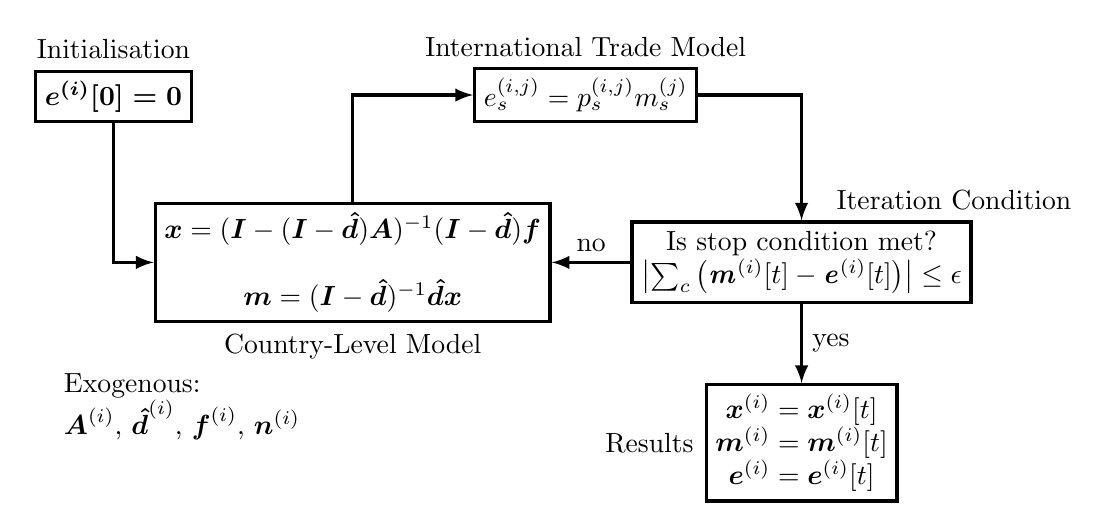
\begin{tikzpicture}[>=latex, very thick]
	\tikzstyle{all nodes}=[shape=rectangle]
	\tikzstyle{box}=[draw]
	% % Nodes
	% init
	\node[box,label=above:Initialisation](init)
	{$\boldsymbol{e^{(i)}[0] = 0}$};
	% country-level model
	\node[box, below right= and -.5cm of init, 
		  align=center, label=below:Country-Level Model]
	(country)
	{
		$
		\boldsymbol{x} = 
		(\boldsymbol{I} - 
		(\boldsymbol{I} - \boldsymbol{\hat{d}})
		\boldsymbol{A})^{-1} 
		(\boldsymbol{I} - \boldsymbol{\hat{d}})\boldsymbol{f}
		$ \\\\
		$
		\boldsymbol{m} = 
		(\boldsymbol{I} - 
		\boldsymbol{\hat{d}})^{-1} 
		\boldsymbol{\hat{d}}\boldsymbol{x}
		$
	};
	% international trade model
	\node[box, above right= and -1cm of country](trade)
	[label=above:International Trade Model]
	{
		$e_s^{(i,j)} = p_s^{(i,j)}m_s^{(j)}$
	};
	% iteration condition
	\node[box, right= of country, align=center](iteration)
	[label=60:Iteration Condition]
	{
		Is stop condition met?
		\\
		$
		\left| \sum_{c} \left(\textbf{\textit{m}}^{(i)}[t] -
		\textbf{\textit{e}}^{(i)}[t] \right) \right| \leq \epsilon
		$
	};
	% results
	\node[box, below=of iteration, align=center](result)
	[label=left:Results]
	{
		$\boldsymbol{x}^{(i)}=\boldsymbol{x}^{(i)}[t]$ \\
		$\boldsymbol{m}^{(i)}=\boldsymbol{m}^{(i)}[t]$ \\
		$\boldsymbol{e}^{(i)}=\boldsymbol{e}^{(i)}[t]$
	};
	% Exogenous annotation
	\node[below left=0.5cm and -2cm of country, align=left] {
	Exogenous: \\
	$\boldsymbol{A}^{(i)}$,
	$\boldsymbol{\hat{d}}^{(i)}$,
	$\boldsymbol{f}^{(i)}$,
	$\boldsymbol{n}^{(i)}$
	};
	% % Connectors
	\draw [->] (init) |- (country);
	\draw [->] (country) |- (trade);
	\draw [->] (trade) -| (iteration);
	\draw [->] (iteration) -- node[above]{no} (country);
	\draw [->] (iteration) -- node[right]{yes}(result);
\end{tikzpicture}
\caption{The model algorithm: total production, imports and exports are calculated for a given set of exogenous parameters.}\label{fig:algorithm}
\end{figure}

\section{Analysis}\label{sec:analysis}
The model combining input-output country descriptions and the international trade network allows for the measurement of the total input required to make a single unit of a particular sector's good.
Since the WIOD reports goods flows in millions of US dollars (\$M), this will also be the unit of all the following analysis.

A simple way to measure the efficiency of a sector is to reduce final demand for the goods of that sector by one unit, and measure the response of each other sector in the model. We can formalise the final-demand change in sector $s$ in country $i$ as:

\begin{equation}\label{eqn:reduce_fd_by_one}
f_s^{(i)} \rightarrow f_s^{\prime (i)} \equiv (f_s^{(i)} - 1)
\end{equation}

The simplest way to define `response' is as the change of total output of all sectors, $r$, in all countries, $j$, caused by the reduction:
\begin{equation}
\Delta x_{sr}^{(ij)} \equiv (x_{sr}^{\prime(ij)} - x_r^{(j)})
\end{equation}
where $x_{sr}^{\prime(ij)}$ is the total output of sector $r$ in country $j$ after the change in equation \eqref{eqn:reduce_fd_by_one} has taken place and the model has been recalculated according to Figure \ref{fig:algorithm}.
$\Delta x_{sr}^{(ij)}$ is thus the change in output of sector $r$ in country $j$ induced by the change in final demand for sector $s$ in country $i$.

The total response induced by sector $s$ in country $i$ is:
\begin{equation}
\eta_s^{(i)} \equiv \Delta x_{s}^{(i)} = \sum_j \sum_r \Delta x_{sr}^{(ij)}
\end{equation}
and the average response across all sectors in country $i$ is:
\begin{equation}
\eta^{(i)} = \frac{\sum_s \eta_s^{(i)}}{S}
\end{equation}
where $S$ is the number of sectors in country $i$'s economy.

Sectors with a larger value of $\eta_s^{(i)}$ require a larger amount of input to produce each unit of their output compared with other sectors. $\eta{(i)}$ can thus be thought of as an (in)efficiency measure, with larger values implying a less-efficient production technology on average across all sectors.

Figure \ref{tbl:least_efficient_countries} shows the 10 least efficient countries by this measure.
China is the world's least efficient producer, a \$1M reduction in final demand leading to an average \$2.36M reduction in total output worldwide.
 
This is perhaps a surprising result.
To investigate further, the efficiency measure, $\eta^{(i)}$ can be divided into foreign and domestic effects, as follows:

\begin{align}
\eta_s^{*(i)} \equiv \Delta x_{s}^{*(i)} & = 
	\sum_{j \neq i} \sum_r \Delta x_{sr}^{(ij)} \\
\eta^{*(i)} & = 
	\frac{\sum_s \eta_s^{*(i)}}{S}
\end{align}
and
\begin{align}
\eta_s^{\dagger(i)} \equiv \Delta x_{s}^{\dagger(i)} & = 
	\sum_r \Delta x_{sr}^{(ii)} \\
\eta^{\dagger(i)} & = 
	\frac{\sum_s \eta_s^{\dagger(i)}}{S}
\end{align}
such that
\begin{equation}
\eta^{(i)} = \eta^{*(i)} + \eta^{\dagger(i)}
\end{equation}
Figure \ref{fig:countries_domestic_vs_foreign} shows how the average response across all sectors divides between domestic response, $\eta_s^{\dagger}$, and foreign response, $\eta_s^{*}$, for each country. 
An OLS regression line has been added to the plot, and the grey shaded area represents the 5\% confidence interval.
Countries which lie close to the line all have a similar total efficiency, $\eta^{(i)}$.
The region below the line is the region of greater-than-average efficiency and that above the line is the region of smaller-than-average efficiency.
Countries further to the left, such as Brazil, India, Japan, Russia, Turkey and the USA, are more self-reliant than those on the right, such as Luxembourg, Belgium, the Netherlands and Denmark.
This self-reliance can be made precise by measuring the ratio of domestic response to foreign response:

\begin{equation}
\phi^{(i)} = \frac{\eta^{*(i)}}{\eta^{\dagger(i)}}
\end{equation}

China is immediately visible as an outlier.
Its production technology is around one-third less efficient ($\eta = 2.36$) than that of Brazil ($\eta = 1.75$) or India ($\eta = 1.74$), but almost all of this extra inefficiency in targeted at domestic sectors.
Thus China's production inefficiencies benefit its domestic sectors to a disproportionate extent.

\begin{figure}
	\centering
	\subfigure[least efficient countries]
	{
		\begin{tabular}{lr}
		\toprule
		Country & Production efficiency, $\eta^{(i)}$\\
		\midrule
          China &       2.36 \\
 Czech Republic &       1.98 \\
       S. Korea &       1.95 \\
         Russia &       1.94 \\
       Bulgaria &       1.92 \\
          Japan &       1.90 \\
          Italy &       1.90 \\
         Poland &       1.89 \\
        Finland &       1.88 \\
       Portugal &       1.87 \\
		\bottomrule
		\end{tabular}
		\label{tbl:least_efficient_countries}
	}
	\subfigure[China's least efficient sectors]
	{
		\begin{tabular}{lr}
		\toprule
		       Sector & Production efficiency, $\eta_s^{(\text{China})}$\\
		\midrule
		     Vehicles &       2.47 \\
		         Food &       2.20 \\
		     Plastics &       2.20 \\
		       Metals &       2.17 \\
		    Machinery &       2.17 \\
		         Wood &       2.14 \\
		  Electricals &       2.13 \\
		 Construction &       2.12 \\
		     Textiles &       2.11 \\
		        Paper &       2.10 \\
		\bottomrule
		\end{tabular}
		\label{tbl:chinas_least_efficient_sectors}
	}
	\caption{Response to a \$1M reduction in final demand, in terms of difference induced in the total output, $x$, of other sectors. Only the largest 10 are shown.}
\end{figure}

\begin{figure}
\centering
\includegraphics[width=\textwidth]{"images/country response domestic vs foreign - tweaked".pdf}
\caption{The total response of the global economy to a reduction in final demand, averaged across every sector in a country. 
`Response' is defined as the total production lost across all sectors.
Here, response has been divided into domestic, where the response is measured only in the country whose final demand has been reduced, and foreign, where the response is measured in all other countries only.
The solid line shows the result of an OLS regression, with the grey shaded area being the 5\% confidence interval.}
\label{fig:countries_domestic_vs_foreign}
\end{figure}

\subsection*{A unified network approach}
The flow of goods between countries can be viewed as a weighted, directed network, where countries are nodes, and the weights of each edge represents the magnitude of the flow between them \parencite{Nystuen1961,Serrano2003,Bhattacharya2008,Baskaran2011}.
Similarly with the sector-sector flows which constitute an input-output model \parencite{Blochl2011}.
Network science has developed useful ways to analyse the sort of weighted, directed networks which the constitute the present model, but a single network representation is required which combines the international and the sub-national networks.

Recall from section \ref{sec:importratios} above, that goods arriving at the shores of an importing country are put into a warehouse along with domestically produced goods, at which point the two become indistinguishable.
If an additional assumption is made that domestic sectors take from this warehouse by method of a random sample, then the fraction of goods in each sample from abroad will be identical, as will the fraction of imported goods from each exporter.
These fractions will be set by the import ratios and import propensities respectively.

This additional assumption allows us to specify a complete system of intermediate (input-output) flows, $y_{rs}^{(i,j)}$, from sector $r$ in country $i$ to sector $s$ in country $j$:

\begin{equation}\label{eqn:y_rsij}
y_{rs}^{(i,j)} = p_{r}^{(i,j)} d_{r}^{(j)} a_{rs}^{(j)} x_{s}^{(j)}
\end{equation}
Equation \eqref{eqn:y_rsij} can be understood as follows:
sector $s$ in country $j$ requires an amount $a_{rs}^{(j)} x_{s}^{(j)}$ of sector $r$'s good to produce its total output;
a fraction $d_{r}^{(j)}$ of this will be supplied by imports;
a fraction $p_{r}^{(i,j)}$ of these imports will come from country $i$. Note that since countries do not import their own exports, $p_s^{(i,i)}=0,\ \forall i$, and the expression holds trivially for $i=j$.

The fractions of each type of demand for $s$ in country $j$ which was exported by country $i$ are given by similar expressions:

\begin{subequations}
\begin{equation}\label{eqn:y_rsij}
f_{s}^{(i,j)} = p_{s}^{(i,j)} d_{s}^{(j)} f_{s}^{(j)}
\end{equation}
\begin{equation}\label{eqn:y_rsij}
e_{s}^{(i,j)} = p_{s}^{(i,j)} d_{s}^{(j)} e_{s}^{(j)}
\end{equation}
\begin{equation}\label{eqn:y_rsij}
n_{s}^{(i,j)} = p_{s}^{(i,j)} d_{s}^{(j)} n_{s}^{(j)}
\end{equation}
\end{subequations}
where, as previously, $f$ is final demand, $e$ is export demand and $n$ are investments.

Along with the sector-to-sector flows given by equation \eqref{eqn:zstar}, this allows the representation of all the flows in the present model as a single network, and standard network analysis techniques can then be used.

We can visualise the changes which occur following the reduction of demand in China for the Vehicles sector by \$1M. The change to every flow (both $y_{rs}^{(i,j)}$ and $z_{rs}^{(i)}$ type flows) is recorded and visualised in figure \ref{fig:chnvehtop6}.

\begin{figure}
\centering
\includegraphics[width=\textwidth]{"images/Chinese Vehicles Top 10 Countries".png}
\caption{A network representation of the seven most-affected countries following a reduction in final demand for the Chinese vehicles sector. Node size is proportional to eigenvector centrality, and edge width is proportional to the change in flow.}\label{fig:chnvehtop6}
\end{figure}


\section{Conclusions}\label{sec:conclusions}

\printbibliography

\end{document} 
